%%
% Copyright (c) 2017 - 2020, Pascal Wagler;
% Copyright (c) 2014 - 2020, John MacFarlane
%
% All rights reserved.
%
% Redistribution and use in source and binary forms, with or without
% modification, are permitted provided that the following conditions
% are met:
%
% - Redistributions of source code must retain the above copyright
% notice, this list of conditions and the following disclaimer.
%
% - Redistributions in binary form must reproduce the above copyright
% notice, this list of conditions and the following disclaimer in the
% documentation and/or other materials provided with the distribution.
%
% - Neither the name of John MacFarlane nor the names of other
% contributors may be used to endorse or promote products derived
% from this software without specific prior written permission.
%
% THIS SOFTWARE IS PROVIDED BY THE COPYRIGHT HOLDERS AND CONTRIBUTORS
% "AS IS" AND ANY EXPRESS OR IMPLIED WARRANTIES, INCLUDING, BUT NOT
% LIMITED TO, THE IMPLIED WARRANTIES OF MERCHANTABILITY AND FITNESS
% FOR A PARTICULAR PURPOSE ARE DISCLAIMED. IN NO EVENT SHALL THE
% COPYRIGHT OWNER OR CONTRIBUTORS BE LIABLE FOR ANY DIRECT, INDIRECT,
% INCIDENTAL, SPECIAL, EXEMPLARY, OR CONSEQUENTIAL DAMAGES (INCLUDING,
% BUT NOT LIMITED TO, PROCUREMENT OF SUBSTITUTE GOODS OR SERVICES;
% LOSS OF USE, DATA, OR PROFITS; OR BUSINESS INTERRUPTION) HOWEVER
% CAUSED AND ON ANY THEORY OF LIABILITY, WHETHER IN CONTRACT, STRICT
% LIABILITY, OR TORT (INCLUDING NEGLIGENCE OR OTHERWISE) ARISING IN
% ANY WAY OUT OF THE USE OF THIS SOFTWARE, EVEN IF ADVISED OF THE
% POSSIBILITY OF SUCH DAMAGE.
%%

%%
% This is the Eisvogel pandoc LaTeX template.
%
% For usage information and examples visit the official GitHub page:
% https://github.com/Wandmalfarbe/pandoc-latex-template
%%

% Options for packages loaded elsewhere
\PassOptionsToPackage{unicode}{hyperref}
\PassOptionsToPackage{hyphens}{url}
\PassOptionsToPackage{dvipsnames,svgnames*,x11names*,table}{xcolor}
%
\documentclass[
  14pt
  american,
  paper=a4,
  ,captions=tableheading
]{scrbook}
\usepackage{amsmath,amssymb}
\usepackage{lmodern}
\usepackage{setspace}
\setstretch{1.2}
\usepackage{amsmath}
\usepackage{ifxetex,ifluatex}
\ifnum 0\ifxetex 1\fi\ifluatex 1\fi=0 % if pdftex
  \usepackage[T1]{fontenc}
  \usepackage[utf8]{inputenc}
  \usepackage{textcomp} % provide euro and other symbols
  \usepackage{amssymb}
\else % if luatex or xetex
  \usepackage{unicode-math}
  \defaultfontfeatures{Scale=MatchLowercase}
  \defaultfontfeatures[\rmfamily]{Ligatures=TeX,Scale=1}
  \setmainfont[]{DejaVu Sans}
  \setmonofont[]{Source Code Pro}
\fi
% Use upquote if available, for straight quotes in verbatim environments
\IfFileExists{upquote.sty}{\usepackage{upquote}}{}
\IfFileExists{microtype.sty}{% use microtype if available
  \usepackage[]{microtype}
  \UseMicrotypeSet[protrusion]{basicmath} % disable protrusion for tt fonts
}{}
\makeatletter
\@ifundefined{KOMAClassName}{% if non-KOMA class
  \IfFileExists{parskip.sty}{%
    \usepackage{parskip}
  }{% else
    \setlength{\parindent}{0pt}
    \setlength{\parskip}{6pt plus 2pt minus 1pt}}
}{% if KOMA class
  \KOMAoptions{parskip=half}}
\makeatother
\usepackage{xcolor}
\definecolor{default-linkcolor}{HTML}{A50000}
\definecolor{default-filecolor}{HTML}{A50000}
\definecolor{default-citecolor}{HTML}{4077C0}
\definecolor{default-urlcolor}{HTML}{4077C0}
\IfFileExists{xurl.sty}{\usepackage{xurl}}{} % add URL line breaks if available
\IfFileExists{bookmark.sty}{\usepackage{bookmark}}{\usepackage{hyperref}}
\hypersetup{
  pdftitle={Tools for Science},
  pdfauthor={Rik Huijzer},
  pdflang={en-US},
  colorlinks=true,
  linkcolor=blue,
  filecolor=default-filecolor,
  citecolor=default-citecolor,
  urlcolor=default-urlcolor,
  breaklinks=true,
  pdfcreator={LaTeX via pandoc with the Eisvogel template}}
\urlstyle{same} % disable monospaced font for URLs
\usepackage[top=20mm,left=24mm,right=24mm,bottom=28mm]{geometry}
\usepackage{listings}
\newcommand{\passthrough}[1]{#1}
\lstset{defaultdialect=[5.3]Lua}
\lstset{defaultdialect=[x86masm]Assembler}
\usepackage{longtable,booktabs,array}
\usepackage{calc} % for calculating minipage widths
% Correct order of tables after \paragraph or \subparagraph
\usepackage{etoolbox}
\makeatletter
\patchcmd\longtable{\par}{\if@noskipsec\mbox{}\fi\par}{}{}
\makeatother
% Allow footnotes in longtable head/foot
\IfFileExists{footnotehyper.sty}{\usepackage{footnotehyper}}{\usepackage{footnote}}
\makesavenoteenv{longtable}
% add backlinks to footnote references, cf. https://tex.stackexchange.com/questions/302266/make-footnote-clickable-both-ways
\usepackage{footnotebackref}
\usepackage{graphicx}
\makeatletter
\def\maxwidth{\ifdim\Gin@nat@width>\linewidth\linewidth\else\Gin@nat@width\fi}
\def\maxheight{\ifdim\Gin@nat@height>\textheight\textheight\else\Gin@nat@height\fi}
\makeatother
% Scale images if necessary, so that they will not overflow the page
% margins by default, and it is still possible to overwrite the defaults
% using explicit options in \includegraphics[width, height, ...]{}
\setkeys{Gin}{width=\maxwidth,height=\maxheight,keepaspectratio}
% Set default figure placement to htbp
\makeatletter
\def\fps@figure{htbp}
\makeatother
\setlength{\emergencystretch}{3em} % prevent overfull lines
\providecommand{\tightlist}{%
  \setlength{\itemsep}{0pt}\setlength{\parskip}{0pt}}
\setcounter{secnumdepth}{5}

% Make use of float-package and set default placement for figures to H.
% The option H means 'PUT IT HERE' (as  opposed to the standard h option which means 'You may put it here if you like').
\usepackage{float}
\floatplacement{figure}{H}

\makeatletter
\@ifpackageloaded{subfig}{}{\usepackage{subfig}}
\@ifpackageloaded{caption}{}{\usepackage{caption}}
\captionsetup[subfloat]{margin=0.5em}
\AtBeginDocument{%
\renewcommand*\figurename{Figure}
\renewcommand*\tablename{Table}
}
\AtBeginDocument{%
\renewcommand*\listfigurename{List of Figures}
\renewcommand*\listtablename{List of Tables}
}
\newcounter{pandoccrossref@subfigures@footnote@counter}
\newenvironment{pandoccrossrefsubfigures}{%
\setcounter{pandoccrossref@subfigures@footnote@counter}{0}
\begin{figure}\centering%
\gdef\global@pandoccrossref@subfigures@footnotes{}%
\DeclareRobustCommand{\footnote}[1]{\footnotemark%
\stepcounter{pandoccrossref@subfigures@footnote@counter}%
\ifx\global@pandoccrossref@subfigures@footnotes\empty%
\gdef\global@pandoccrossref@subfigures@footnotes{{##1}}%
\else%
\g@addto@macro\global@pandoccrossref@subfigures@footnotes{, {##1}}%
\fi}}%
{\end{figure}%
\addtocounter{footnote}{-\value{pandoccrossref@subfigures@footnote@counter}}
\@for\f:=\global@pandoccrossref@subfigures@footnotes\do{\stepcounter{footnote}\footnotetext{\f}}%
\gdef\global@pandoccrossref@subfigures@footnotes{}}
\@ifpackageloaded{float}{}{\usepackage{float}}
\floatstyle{ruled}
\@ifundefined{c@chapter}{\newfloat{codelisting}{h}{lop}}{\newfloat{codelisting}{h}{lop}[chapter]}
\floatname{codelisting}{Listing}
\newcommand*\listoflistings{\listof{codelisting}{List of Listings}}
\makeatother
\ifxetex
      % Load polyglossia as late as possible: uses bidi with RTL langages (e.g. Hebrew, Arabic)
  \usepackage{polyglossia}
  \setmainlanguage[variant=american]{english}
\else
  \usepackage[main=american]{babel}
% get rid of language-specific shorthands (see #6817):
\let\LanguageShortHands\languageshorthands
\def\languageshorthands#1{}
\fi
\ifluatex
  \usepackage{selnolig}  % disable illegal ligatures
\fi

% From the Pandoc default template for 2.11.4.
\newlength{\cslhangindent}
\setlength{\cslhangindent}{1.5em}
\newlength{\csllabelwidth}
\setlength{\csllabelwidth}{3em}
\newenvironment{CSLReferences}[2] % #1 hanging-ident, #2 entry spacing
 {% don't indent paragraphs
  \setlength{\parindent}{0pt}
  % turn on hanging indent if param 1 is 1
  \ifodd #1 \everypar{\setlength{\hangindent}{\cslhangindent}}\ignorespaces\fi
  % set entry spacing
  \ifnum #2 > 0
  \setlength{\parskip}{#2\baselineskip}
  \fi
 }%
 {}
\usepackage{calc}
\newcommand{\CSLBlock}[1]{#1\hfill\break}
\newcommand{\CSLLeftMargin}[1]{\parbox[t]{\csllabelwidth}{#1}}
\newcommand{\CSLRightInline}[1]{\parbox[t]{\linewidth - \csllabelwidth}{#1}\break}
\newcommand{\CSLIndent}[1]{\hspace{\cslhangindent}#1}

\title{Tools for Science}
\usepackage{etoolbox}
\makeatletter
\providecommand{\subtitle}[1]{% add subtitle to \maketitle
  \apptocmd{\@title}{\par {\large #1 \par}}{}{}
}
\makeatother
\subtitle{Automate work and manage complexity}
\author{Rik Huijzer}
\date{}



%%
%% added
%%

%
% language specification
%
% If no language is specified, use English as the default main document language.
%



%
% for the background color of the title page
%
\usepackage{pagecolor}
\usepackage{afterpage}

%
% break urls
%
\PassOptionsToPackage{hyphens}{url}

%
% When using babel or polyglossia with biblatex, loading csquotes is recommended
% to ensure that quoted texts are typeset according to the rules of your main language.
%
\usepackage{csquotes}

%
% captions
%
\definecolor{caption-color}{HTML}{777777}
\usepackage[font={stretch=1.2}, textfont={color=caption-color}, position=top, skip=4mm, labelfont=bf, singlelinecheck=false, justification=raggedright]{caption}

%
% blockquote
%
\definecolor{blockquote-border}{RGB}{221,221,221}
\definecolor{blockquote-text}{RGB}{119,119,119}
\usepackage{mdframed}
\newmdenv[rightline=false,bottomline=false,topline=false,linewidth=3pt,linecolor=blockquote-border,skipabove=\parskip]{customblockquote}
\renewenvironment{quote}{\begin{customblockquote}\list{}{\rightmargin=0em\leftmargin=0em}%
\item\relax\color{blockquote-text}\ignorespaces}{\unskip\unskip\endlist\end{customblockquote}}

%
% Source Sans Pro as the de­fault font fam­ily
% Source Code Pro for monospace text
%
% 'default' option sets the default
% font family to Source Sans Pro, not \sfdefault.
%

\ifnum 0\ifxetex 1\fi\ifluatex 1\fi=0 % if pdftex
    \else % if not pdftex
    \fi

%
% heading color
%
\definecolor{heading-color}{RGB}{40,40,40}
% \addtokomafont{section}{\color{heading-color}}
% When using the classes report, scrreprt, book,
% scrbook or memoir, uncomment the following line.
% \addtokomafont{chapter}{\color{heading-color}}

%
% variables for title, author and date
%
\usepackage{titling}
\title{Tools for Science}
\author{Rik Huijzer}
\date{}

%
% tables
%

\definecolor{table-row-color}{HTML}{F5F5F5}
\definecolor{table-rule-color}{HTML}{999999}

%\arrayrulecolor{black!40}
\arrayrulecolor{table-rule-color}     % color of \toprule, \midrule, \bottomrule
\setlength\heavyrulewidth{0.3ex}      % thickness of \toprule, \bottomrule
\renewcommand{\arraystretch}{1.3}     % spacing (padding)


%
% remove paragraph indention
%
\setlength{\parindent}{0pt}
\setlength{\parskip}{6pt plus 2pt minus 1pt}
\setlength{\emergencystretch}{3em}  % prevent overfull lines

%
%
% Listings
%
%

%
% general listing colors
%
\definecolor{listing-background}{HTML}{F7F7F7}
\definecolor{listing-rule}{HTML}{B3B2B3}
\definecolor{listing-numbers}{HTML}{B3B2B3}
\definecolor{listing-text-color}{HTML}{080808}
\definecolor{listing-keyword}{HTML}{435489}
\definecolor{listing-keyword-2}{HTML}{1284CA} % additional keywords
\definecolor{listing-keyword-3}{HTML}{9137CB} % additional keywords
\definecolor{listing-identifier}{HTML}{435489}
\definecolor{listing-string}{HTML}{00999A}
\definecolor{listing-comment}{HTML}{8E8E8E}

%
% Better no syntax highlighting than wrong syntax highlighting.
%
\lstdefinelanguage{raw}{
  keywordstyle=\ttfamily
}

\lstdefinestyle{eisvogel_listing_style}{
  language         = raw,
  xleftmargin      = 0.6em,
  framexleftmargin = 0.4em,
  backgroundcolor  = \color{listing-background},
  basicstyle       = \color{listing-text-color}\linespread{1.4}\scriptsize\ttfamily{},
  breaklines       = true,
  frame            = single,
  framesep         = 0.19em,
  rulecolor        = \color{listing-rule},
  frameround       = ffff,
  tabsize          = 4,
  numberstyle      = , % \color{listing-numbers},
  aboveskip        = 0.8em,
  belowskip        = 0.5em,
  abovecaptionskip = 0em,
  belowcaptionskip = 1.0em,
  keywordstyle     = , % {\color{listing-keyword}\bfseries},
  keywordstyle     = , % {[2]\color{listing-keyword-2}\bfseries},
  keywordstyle     = , % {[3]\color{listing-keyword-3}\bfseries\itshape},
  sensitive        = true,
  identifierstyle  = , % \color{listing-identifier},
  commentstyle     = , % \color{listing-comment},
  stringstyle      = , % \color{listing-string},
  showstringspaces = false,
  escapeinside     = {/*@}{@*/}, % Allow LaTeX inside these special comments
  literate         =
  {á}{{\'a}}1 {é}{{\'e}}1 {í}{{\'i}}1 {ó}{{\'o}}1 {ú}{{\'u}}1
  {Á}{{\'A}}1 {É}{{\'E}}1 {Í}{{\'I}}1 {Ó}{{\'O}}1 {Ú}{{\'U}}1
  {à}{{\`a}}1 {è}{{\'e}}1 {ì}{{\`i}}1 {ò}{{\`o}}1 {ù}{{\`u}}1
  {À}{{\`A}}1 {È}{{\'E}}1 {Ì}{{\`I}}1 {Ò}{{\`O}}1 {Ù}{{\`U}}1
  {ä}{{\"a}}1 {ë}{{\"e}}1 {ï}{{\"i}}1 {ö}{{\"o}}1 {ü}{{\"u}}1
  {Ä}{{\"A}}1 {Ë}{{\"E}}1 {Ï}{{\"I}}1 {Ö}{{\"O}}1 {Ü}{{\"U}}1
  {â}{{\^a}}1 {ê}{{\^e}}1 {î}{{\^i}}1 {ô}{{\^o}}1 {û}{{\^u}}1
  {Â}{{\^A}}1 {Ê}{{\^E}}1 {Î}{{\^I}}1 {Ô}{{\^O}}1 {Û}{{\^U}}1
  {œ}{{\oe}}1 {Œ}{{\OE}}1 {æ}{{\ae}}1 {Æ}{{\AE}}1 {ß}{{\ss}}1
  {ç}{{\c c}}1 {Ç}{{\c C}}1 {ø}{{\o}}1 {å}{{\r a}}1 {Å}{{\r A}}1
  {€}{{\EUR}}1 {£}{{\pounds}}1 {«}{{\guillemotleft}}1
  {»}{{\guillemotright}}1 {ñ}{{\~n}}1 {Ñ}{{\~N}}1 {¿}{{?`}}1
  {…}{{\ldots}}1 {≥}{{>=}}1 {≤}{{<=}}1 {„}{{\glqq}}1 {“}{{\grqq}}1
  {”}{{''}}1
}
\lstset{style=eisvogel_listing_style}

%
% Java (Java SE 12, 2019-06-22)
%
\lstdefinelanguage{Java}{
  morekeywords={
    % normal keywords (without data types)
    abstract,assert,break,case,catch,class,continue,default,
    do,else,enum,exports,extends,final,finally,for,if,implements,
    import,instanceof,interface,module,native,new,package,private,
    protected,public,requires,return,static,strictfp,super,switch,
    synchronized,this,throw,throws,transient,try,volatile,while,
    % var is an identifier
    var
  },
  morekeywords={[2] % data types
    % primitive data types
    boolean,byte,char,double,float,int,long,short,
    % String
    String,
    % primitive wrapper types
    Boolean,Byte,Character,Double,Float,Integer,Long,Short
    % number types
    Number,AtomicInteger,AtomicLong,BigDecimal,BigInteger,DoubleAccumulator,DoubleAdder,LongAccumulator,LongAdder,Short,
    % other
    Object,Void,void
  },
  morekeywords={[3] % literals
    % reserved words for literal values
    null,true,false,
  },
  sensitive,
  morecomment  = [l]//,
  morecomment  = [s]{/*}{*/},
  morecomment  = [s]{/**}{*/},
  morestring   = [b]",
  morestring   = [b]',
}

\lstdefinelanguage{XML}{
  morestring      = [b]",
  moredelim       = [s][\bfseries\color{listing-keyword}]{<}{\ },
  moredelim       = [s][\bfseries\color{listing-keyword}]{</}{>},
  moredelim       = [l][\bfseries\color{listing-keyword}]{/>},
  moredelim       = [l][\bfseries\color{listing-keyword}]{>},
  morecomment     = [s]{<?}{?>},
  morecomment     = [s]{<!--}{-->},
  commentstyle    = \color{listing-comment},
  stringstyle     = \color{listing-string},
  identifierstyle = \color{listing-identifier}
}

%
% header and footer
%
\usepackage{fancyhdr}

\fancypagestyle{eisvogel-header-footer}{
  \fancyhead{}
  \fancyfoot{}
  \lhead[]{Tools for Science}
  \chead[]{}
  \rhead[Tools for Science]{}
  \cfoot[]{}
  \rfoot[\url{https://github.com/rikhuijzer/tools} ]{\thepage}
  \renewcommand{\headrulewidth}{0.4pt}
  \renewcommand{\footrulewidth}{0.4pt}
}
\pagestyle{eisvogel-header-footer}

%%
%% end added
%%

\begin{document}

%%
%% begin titlepage
%%
\begin{titlepage}
\newgeometry{left=6cm}
\newcommand{\colorRule}[3][black]{\textcolor[HTML]{#1}{\rule{#2}{#3}}}
\begin{flushleft}
\noindent
\\[-1em]
\color[HTML]{5F5F5F}
\makebox[0pt][l]{\colorRule[435488]{1.3\textwidth}{4pt}}
\par
\noindent

{
  \setstretch{1.4}
  \vfill
  \noindent {\huge \textbf{\textsf{Tools for Science}}}
    \vskip 1em
  {\Large \textsf{Automate work and manage complexity}}
    \vskip 2em
  \noindent {\Large \textsf{Rik Huijzer}}
  \vfill
}
{\footnotesize
Creative Commons Attribution-ShareAlike 4.0 International (CC BY-SA 4.0)
}
\textsf{}
\end{flushleft}
\end{titlepage}
\restoregeometry

%%
%% end titlepage
%%

% \frontmatter


{
\hypersetup{linkcolor=}
\setcounter{tocdepth}{2}
\tableofcontents
}
% \mainmatter
\hypertarget{sec:preface}{%
\chapter{Preface}\label{sec:preface}}

Artificial intelligence (AI) is lauded by many as the fourth industrial
revolution. It promises to make better decisions and can automate more
work. One of the largest countries in the world is spending massive
resources on autonomous driving, urban cognition, medical imaging, voice
intelligence, visual computing, marketing intelligence, video
perception, intelligent supply chains, image perception, smart
education, smart homes and many more
(\protect\hyperlink{ref-wu2020towards}{Wu et al., 2020}). In this sense,
we live in exciting times. However, there is a common held belief that
these automated analyses, machine learning, neural networks and
artificial intelligence can only be achieved by large countries, or
companies like DeepMind, OpenAI, Microsoft, Netflix and Amazon. This is
false. Basically, what we call artificial intelligence is just machine
learning (\protect\hyperlink{ref-jordan2019artificial}{Jordan, 2019})
which is basically statistics. Here, it is statistics being applied by
software engineers. The benefit of software engineerings is that they
are used to managing complexity with tools. So, for software engineers
it doesn't matter they work on the newest maching learning systems or
more traditional systems. In both cases, the work is quite similar.

There have been failures with AI software, such as Microsoft's chatbot
learning offensive language or Apple's Face ID being broken by hackers
(\protect\hyperlink{ref-greenberg2017hackers}{Greenberg, 2017}). Still,
it is mostly success stories about beating the world champion in Go
matches (\protect\hyperlink{ref-deepmind2020alphago}{DeepMind, 2020}),
predicting the stock market, selling more products with better
recommendations. The success comes from the scaling capabilities. Once
the software is correct, it can be scaled to millions of users or base
analysis results on petabytes of data.

However, software engineering isn't part of the typical scientist's
skillset. Non-engineering students are taught to do statistical analyses
in convenient statistical software with graphical user interfaces, such
as Excel, SPSS, JAGS or JASP. The problem with these tools is that they
cannot solve any computation problem. In their daily life, they will run
into problems which are out of the scope of these convenient tools. This
while the \textbf{real} tools, general-purpose programming lanuages,
have never been easier to use. Everything you need to automate analyses
and work with AI is publicly and freely available.

This explains why I decided to write this book. With a background in
computer science, I have transitioned to a PhD in Psychology. Here, I
see that days are fully spent behind a computer while being hindered by
the convenient tools. I hear the same stories from colleagues in the
medical, biological, chemical and mathematical sciences. I've even heard
professors talk about some of their tasks being laborious while knowing
that many great tools can easily automate these tasks. Unfortunately, I
know that using these tools cannot be learned in a day; learning only
one of them is not enough. Combining the tools in this book is where the
real power lies. I've often convinced people of some tool by amazing
them with the speed. However, on their way home, they would realise that
the tool doesn't work in their workflow. That's why I wrote this book:
to show the whole picture instead of just one tool. Also, with this book
I aim to present the essentials. These essentials will remain applicable
for many years to come and allow you to easily switch to other tools.

\hypertarget{audience}{%
\section{Audience}\label{audience}}

This book is aimed at scientists. Actually, most chapters will work for
most office jobs, but the book is written with scientists in mind. This
book shows you the tools to get rid of your tedious tasks and how to
manage complexity effectively with the proper software. Software can do
this for you because if you read this on a electronic device, then you
probably don't know how the transistors, registors, instruction sets,
assembly code or application code works. However, this complexity is all
hidden away for you and you can assume all parts to do the work for you.

\hypertarget{reading-this-book}{%
\section{Reading this book}\label{reading-this-book}}

The chapters will build on top of each other in the sense that later
chapters are easier when the tools of easier chapters are used. Also,
I've tried to order the chapters by decreasing importance. For example,
later chapters include more code which is managed best via version
control. Some people will say that this book is too extreme; some of the
presented tools could be replaced by a more beginner friendly version.
Unfortunately, those friendlier versions will not teach you the basics.
It will be easy to switch from the tools in this book to friendlier
versions, but not the reverse. Also, friendlier tools are friendlier by
assuming things for you. This is nice if you want to stick to their
conventions, but if you want something outside of what they provide,
you're out of luck. Then, the only way to get it is to go back to the
more basic tools or to ask the developer to implement your feature.
Also, these basic tools are used by more other tools and people, so more
effort is put into the development. That, in turn, usually results in
the tools being more reliable, better documented and more performant. As
another argument, these basics will allow you to combine the tools more
easily, giving you more power. Other people will call this book
opinionated, and push for other tools. That is why I've spent a great
amount of arguing for the merits of each tool. If you already use
another similar too and are happy with it, then please skip the chapter
in this book.

\hypertarget{sec:notation}{%
\section{Notation}\label{sec:notation}}

To keep the text short and clear, this book uses mathematical notation.
For example, instead of ``the mean for the random samples equals
three,'' we write

\[ \text{mean}(X) = 3, \]

where \(X\) are the samples or: let \(X\) denote the random samples,
then

\[ \text{mean}(X) = 3. \]

In this book, I tried to keep the notation consistent, as well as as
close to the code as possible. Therefore, a single value will be denoted
by a lowercase symbol, such as \(x\) and a vector or matrix will be
denoted by an uppercase symbol, such as \(X\). By default, a vector is
assumed to be a column vector like, for example,

\[ X = \begin{bmatrix}
           1 \\
           2 \\
         \end{bmatrix} \]

Or, more generally, a vector of length \(n\) is denoted by

\[ X_{n} = \begin{bmatrix}
           x_1 \\
           x_2 \\
           \vdots \\
           x_n
         \end{bmatrix}, \]

where \(x_1, ..., x_n\) denote single values from the vector \(X\).
Similarily, a matrix with \(n\) rows and \(m\) columns is denoted by
\(X_{n \times m}\). Note that a vector is just a one dimensional matrix;
hence,

\[ X_{n} = X_{n \times 1}. \]

These sizes in the subscript are omitted when possible. Transposition
for a vector or matrix is denoted by \(T\). So, for example,

\[ X_n^T = [ x_1, x_2, ..., x_n ]. \]

For functions, I try to be explicit about the variables, that is, try to
have as little state as possible in the functions. So, for example,
instead of writing a linear model as

\[ y = w_0 + w_1 x, \]

or

\[ y(X) = w_0 + w_1 x_1, \]

I favor

\[ \text{lm}(X, W) = w_0 + w_1 x_1, \]

where \(\text{lm}\) could be any name. On top of this, I will
respectively use Greek and Latin letters for measures of the population
and samples since this is a common convention in statistics
(\protect\hyperlink{ref-smith2018mathematical}{Smith, 2018}).

\hypertarget{acknowledgements}{%
\section{Acknowledgements}\label{acknowledgements}}

Many people have contributed directly and indirectly to this book. My
PhD supervisors have allowed me to do my work with any tools I prefer.
This allowed me to experiment with different tools while keeping in mind
that things have to get done.

\hypertarget{sec:start}{%
\chapter{Where it all starts}\label{sec:start}}

For most scientists, the biggest part of the work isn't in the lab or in
the field. It is, basically, moving text and data around. By this, I
mean that reports have to be written and updated, data has to be
cleaned, and analyses have to be run, updated and re-run.

To do so effectively, Section~\ref{sec:interacting} argues that you
should primarily focus on interacting with the computer via text, and
this is demonstrated in Section~\ref{sec:command-line}.

\hypertarget{sec:interacting}{%
\section{Interacting via text}\label{sec:interacting}}

To get things done on a computer effectively, the focus should be on
interacting with it via text. There are multiple reasons for this.
Firstly, the number of things you can express with text scales
exponentially with the number of words. For instance: given 26 letters
in the alphabet, you can express \(26\) different things with one
letter, \(26 \cdot 26\) different things with two letters, to \(26^n\)
different things with \(n\) letters; also known as ordered sampling with
replacement. So, suppose all the programs in the world are required to
be 7 letters, like \passthrough{\lstinline!bigtree!}, and all the
programs take 3 letters of input. Then, you can choose from
\(26 \cdot 7 = 8.0 \cdot 10^9\) programs, and each program can take
\(26^3 \approx 17.500\) different inputs. Imagine having
\(8.0 \cdot 10^9\) icons on your desktop and, after opening a program,
being presented with \(17.500\) buttons. Another benefit of text is that
you can exchange it easily via online communications. A tutorial for a
text-based tool includes sentences such as:

\begin{quote}
After that, run

\begin{lstlisting}
move A B
\end{lstlisting}
\end{quote}

whereas, graphical user interface users have to rely on tutorials such
as:

\begin{quote}
After that, click on the ``tools'' button in the menu. Then, click on
``move'' and drag \passthrough{\lstinline!A!} to
\passthrough{\lstinline!B!} in the window.
\end{quote}

which is confusing and verbose. Another argument is that text is ``the
most powerful, useful, effective communication technology'' because it
(\protect\hyperlink{ref-hoare2014bet}{Hoare, 2014})

\begin{itemize}
\tightlist
\item
  is the most stable, that is, can be read in many years from now,
\item
  can express many (abstract) things which can't be expressed in images
  such as ``Human rights are moral principles'' and
\item
  is the most efficient communication technology.
\end{itemize}

Finally, tools are written in code, which is basically text. Therefore,
the default interface between tools is text, and a GUI is often just a
layer on top. In the best case, software built on top of of other
software implements all features, but usually the upper layers only
contain a subset. From experience, I know that it is extremely
frustrating to find these boundaries. Usually, you only find these after
investing a lot of time in a tool, and it means that you have migrate
your existing project to another tool. This is a bit like building your
house from construction plans; only to realise halfway the project that
the plan doesn't include a bathroom and that you have to switch over to
other construction plans.

\hypertarget{sec:command-line}{%
\section{Command line}\label{sec:command-line}}

Before operating systems, such as Microsoft Windows, Apple MacOS and
Linux, included fancy graphical user interfaces based around icons, the
mouse and draggable windows, all the work was done from the terminal.
For example, an MS-DOS computer booting into something looking like

\begin{lstlisting}
MS-DOS version 4.00
Copyright 1981,82,83,84,85 Microsoft Corp.

C>echo Hello
Hello
\end{lstlisting}

From this terminal, you could do anything you want. You could start
programs, move files, edit spreadsheets and send documents to printers.
However, although this is quite powerful, it is also unwieldy because
the most basic terminals only allow you to do one tasks at the same
time. Also, browsing the web is difficult, because it is full of
pictures and moving elements which can't be represented nicely via text.
That is why modern operating systems, by default, are built around the
graphical user interface and still allow you to run something which
looks like a terminal in a window. This is also known as a
\emph{terminal emulator}. The terminal emulator allows you to execute
commands. Specifically, it allows you to type a command which the system
will then run. Next, it will show you the output on the next line(s).
For example, to make a directory on Windows called
\passthrough{\lstinline!analysis!} and rename it to
\passthrough{\lstinline!old-analysis!}, you can do

\begin{lstlisting}
Microsoft Windows [Version 10.0.18363.1316]
(c) 2019 Microsoft Corporation. All rights reserved.

C:\Users\John> mkdir tmp

C:\Users\John> cd tmp

C:\Users\John\tmp> mkdir analyis

C:\Users\John\tmp> dir
[...]
04/01/2021  09:36 PM     <DIR>     analysis
[...]

C:\Users\John\tmp> rename analysis old-analysis

C:\Users\John\tmp> dir
[...]
04/01/2021  09:36 PM     <DIR>     old-analysis
[...]
\end{lstlisting}

This behaviour with commands and its output on new lines is why a
terminal emulator is also known as a \emph{command line}. From the
command line, you can start applications via text. In the rest of this
chapter, the book will divert for a bit between operating systems, but
this is only temporarily.

As a simple example, lets open the site of Stanford University in your
favorite browser. In this example, I assume that Firefox is your
favourite browser, but you can also use

\begin{itemize}
\tightlist
\item
  Chrome via \passthrough{\lstinline!chrome!},
\item
  Safari via \passthrough{\lstinline!safari!} \emph{or}
\item
  Edge via \passthrough{\lstinline!msedge!}.
\end{itemize}

\textbf{Windows:}

Start the Command Prompt and type

\begin{lstlisting}
start firefox https://stanford.edu
\end{lstlisting}

\textbf{Apple:}

\ldots{}

\textbf{Linux:}

Start the terminal and type

\begin{lstlisting}
firefox https://stanford.edu
\end{lstlisting}

\hypertarget{commands}{%
\section{Commands}\label{commands}}

If you want to know more about commands, this section will list some
common ones. Otherwise, you can skip this section and come back to it
when you need it.

\hypertarget{sec:git}{%
\chapter{Never losing your files again}\label{sec:git}}

To show why the problem of not losing files is important, lets consider
Kernel-land. In Kernel-land, the people all carry an extensive manual
around which they follow precisely. For instance, when people in this
land want to drink water, they read the according section in the manual
and lift the cup to their mouth only if the manual instructs them to do
so. Also, multiple people carry different manuals, but this is typically
no issue since people can interact happily via conventions, such as
shaking hands when meeting. The main joy in life is attained by
obtaining a newer version of the manual; allowing the Kernel-landers to
do new things and move around the place more quickly.

Now, let's say you and your team are responsible for maintaining and
extending this manual. Maintenance is necessary because the world
changes, so the manual has to be updated accordingly, and extending the
manual is necessary because the people in Kernel-land are getting bored.
At the same time, you try to minimise risks when updating the manual
since earlier changes were disastrous. Once, you have mistakenly changed
the line ``the bananas can be found on the second \emph{aisle} to the
left'' into ``the bananas can be found on the second \emph{isle} to the
left.'' It look quite a lot of work to figure out this bug since the
only practical difference was in the time it took to obtain bananas.

The main complexity of this work is introduced by the size of the
manual. When all working in Word documents, merging the results would be
laborious. By merging, I mean that some team member takes the newest
version of the manual, works on it for a few hours to make changes and
then call this the new version. This works until people start to work on
the document at the same time. Even if the manual is updated in, say,
Section 3 by person A and updated in Section 7 by person B, then these
Word documents are difficult to merge. Without taking care, the person
who saves his version after the other person \emph{wins}. In other
words, the changes of one person will then be overwritten and lost.

Another problem is similar to the problem with the bananas described
above. It can be that one small detail in the manual causes hard to
predict problems. For example, it might happen that Kernellanders report
that the manual tells them to a weird thing like being instructed to
brush their teeth in the nearest house. It can then take a lot of work
to determine that this only happens on rainy afternoons at Sunday in a
town called Sussex, because Sussex is the only place which has 14
streetlights which are all at a 34° angle with the center axis of the
road.

These problems are solved by a tool created by Linus Torvalds. Linus is
the maintainer of the Linux kernel which, in summary, is the manual for
all the Linux computers and servers in the world. Around 2005, Linus had
thousands of people working on the manual
(\protect\hyperlink{ref-loeliger2012version}{Loeliger \& McCullough,
2012}). He was then reviewing the changes and merged them in the main
manual version if it all looked good. A typical merge would take the
computer 2 hours (\protect\hyperlink{ref-torvalds2005}{Torvalds, 2005}),
which Linus wasn't willing to accept. He wanted 3 seconds
(\protect\hyperlink{ref-torvalds2005}{Torvalds, 2005}) which he managed
to obtain by creating \emph{Git}.

Nowadays, Git is the tool that all software engineers agree upon and
where countless other tools are build upon. This is an impressive feat
because there is a joke that says: ``arguing with engineers is like
rolling in the mud with pigs; after a while you realise that they like
it.'' If you talk to software engineers about Git, they will agree that
it is \textbf{the best tool} for the job. Even if you are no software
engineer, this is the tool that has been missing from your life. It will
ensure that you never lose a file and that you don't have to struggle
with files named \passthrough{\lstinline!1!},
\passthrough{\lstinline!1b!}, \passthrough{\lstinline!1b-final!} and
\passthrough{\lstinline!1b-final-final!} again.

\hypertarget{sec:git-history}{%
\section{All your history}\label{sec:git-history}}

\hypertarget{getting-started}{%
\section{Getting started}\label{getting-started}}

To avoid losing files, we want to store our files at multiple computers.
Therefore, we can use Git in combination with GitHub at
\url{https://github.com}. Basically, GitHub is a website built around
Git. If you don't like GitHub, you can also choose to use GitLab
(\url{https://gitlab.com}), Bitbucket (\url{https://bitbucket.org}) or
Gitea (\url{https://gitea.io}). Because these services are built around
the same core, you can easily move your files from one service to the
other if you want. First, we have to create a project to store your
files or a, so called, \emph{repository}. The definition of repository
is ``a place where things may be put for safekeeping''
(\protect\hyperlink{ref-pickett2018american}{Pickett, 2018}). To get
started with GitHub, create an account and a new repository via the
web-interface (\url{https://github.com/new}). You can choose a nice name
and ignore the checkboxes. In this example, we call the repository
\passthrough{\lstinline!novel-paper!} and say that it is created by an
example user called \passthrough{\lstinline!researcher!}. For the rest
of this example, replace \passthrough{\lstinline!novel-paper!} and
\passthrough{\lstinline!researcher!} with respectively your repository
name and username. Next, install Git via the instructions at
\url{https://git-scm.com/downloads}.

Now, the Git robot can be talked to via the terminal. (The terminal is
described in Chapter \ref{sec:start}.) For Git, we need to learn a few
words to handle 99\% of all the use-cases.

First, we have to make a copy of the new repository
\passthrough{\lstinline!novel-paper!} on our own computer so that we can
make changes. Go to a folder where you want to store the repository and
tell the robot to clone the repository:

\begin{lstlisting}
$ git clone https://github.com/example/novel-paper
Cloning into 'novel-paper'...
warning: You appear to have cloned an empty repository.
\end{lstlisting}

or, if you did set one or more of the checkboxes:

\begin{lstlisting}
$ git clone https://github.com/example/novel-paper
remote: Enumerating objects: 3, done.
remote: Counting objects: 100% (3/3), done.
remote: Total 3 (delta 0), reused 0 (delta 0), pack-reused 0
Receiving objects: 100% (3/3), done.
\end{lstlisting}

Your output should look similar to one of these two outputs. Here, Git
told us that some files were received (3 in this case) and everything is
done. In both cases, you will now find a folder called
\passthrough{\lstinline!novel-paper!} and we can start to add a file.
Lets create a ridiciously important file called
\passthrough{\lstinline!ridiciously-important-file.txt!} and place some
text in it

\passthrough{\lstinline!ridiciously-important-file.txt!}:

\begin{lstlisting}
The solution to my research can be found in Devlin & John (2020).
\end{lstlisting}

(And, no, that is not a typo. John can, in fact, be a surname like in
the name Elton John, see \protect\hyperlink{ref-atkinson1991}{Atkinson
\& John} (\protect\hyperlink{ref-atkinson1991}{1991}).)

After doing this, we can see one of the awesome features of the Git
robot. It knows exactly how everything looked before your changes and
can show what has changed. To get a sort of summary of the changes, use

\begin{lstlisting}
$ git status
On branch master

No commits yet

Untracked files:
  (use "git add <file>..." to include in what will be committed)
    ridiciously-important-file.txt

nothing added to commit but untracked files present (use "git add" to track)
\end{lstlisting}

This shows that we have added
\passthrough{\lstinline!ridiciously-important-file.txt!}. To store this
file online, lets \emph{add} all changed files in preparation to pushing
the changes to the server.

\begin{lstlisting}
$ git add .
\end{lstlisting}

This is not definitive yet, we can still check whether everything looks
good:

\begin{lstlisting}
$ git status
On branch master

No commits yet

Changes to be committed:
  (use "git rm --cached <file>..." to unstage)
    new file:   ridiciously-important-file.txt
\end{lstlisting}

As stated in the introduction of this chapter, Git is made to track
complex changes. One way to do this is to describe in words what you're
changing. When the previous \passthrough{\lstinline!git status!} looked
good, we can make these changes permanent, or in other words,
\emph{commit} ourselves to these changes with

\begin{lstlisting}
$ git commit -m 'Add important file'
[master (root-commit) b4f9e1d] Add important file
 1 file changed, 1 insertion(+)
 create mode 100644 ridiciously-important-file.txt
\end{lstlisting}

and \emph{push} them to the server

\begin{lstlisting}
$ git push
Enumerating objects: 3, done.
Counting objects: 100% (3/3), done.
Delta compression using up to 8 threads
Compressing objects: 100% (3/3), done.
Writing objects: 100% (3/3), 303 bytes | 303.00 KiB/s, done.
Total 3 (delta 0), reused 0 (delta 0), pack-reused 0
To https://github.com/researcher/novel-paper
 * [new branch]      master -> master
\end{lstlisting}

You can now see your file online by going to

\begin{lstlisting}
https://github.com/<username>/<repository name>
\end{lstlisting}

\hypertarget{sec:git-collaborating}{%
\section{Collaborating}\label{sec:git-collaborating}}

\hypertarget{sec:editing}{%
\chapter{Quick text editing}\label{sec:editing}}

As an office worker, most of your day is spent on manipulating symbols.
You write papers, reports, notes, presentations, abstracts and maybe use
writing to structure your thoughts. Many of these symbol manipulations
occur often. For instance, think about the number of times that you have
copied or deleted a full sentence, one word, or one or more paragraphs.
Over time, the time and effort spent on these tasks count up.
\protect\hyperlink{ref-yegge2012programmer}{Yegge}
(\protect\hyperlink{ref-yegge2012programmer}{2012}) even tells a story
about how Mailman was an internal application built on top of
\emph{Emacs}, an advanced text editor:

\begin{quote}
People still love it. To this very day, I still have to listen to long
stories from our non-technical folks about how much they miss Mailman.
{[}\ldots{]} Last Christmas I was at an Amazon party, some party I have
no idea how I got invited to, filled with business people, all of them
much prettier and more charming than me and the folks I work with here
in the Furnace, the Boiler Room of Amazon. Four young women found out I
was in Customer Service, cornered me, and talked for fifteen minutes
about how much they missed Mailman and Emacs, and how Arizona (the JSP
replacement we'd spent years developing) still just wasn't doing it for
them.
\end{quote}

This is mostly because these editors help you in getting things done
more quickly. In the rest of this chapter, I will provide a quick-start
for Vi which is roughly the same as Vim
(\href{https://www.vim.org}{www.vim.org}) and Neovim
(\url{https://neovim.io}). Vim is an improved version of Vi and Neovim
is created by a group of developers who weren't happy with Vim and
decided to work on their own copied version. Both editors can be used
mostly interchangibly and that is why I mean Vi, Vim or Neovim when I
mention Vim. I personally prefer Neovim, but Vim works great too. That
this book focusses on Vim doesn't mean that I don't like it's direct
competitor, Emacs. I think both Vim and Emacs can save users tremendeous
amounts of time. For me, Vim seemed more suitable, because it's less
oriented around only a few keys making it less prone to repetitive
strain injury. Also, Emacs wasn't as quick. On the other hand, Emacs has
many great productivity enhancing tools such as Org-mode
(\url{https://orgmode.org}). So, both have their pro's and con's. If
you're unable to do touch typing, then consider reading Chris Wellons'
blog about Vim and touch typing
(\url{https://nullprogram.com/blog/2017/04/01/}).

Vim enhances productivity by introducing different modes. Different
modes allow the behaviour of a key, say \passthrough{\lstinline!d!}, to
change depending on the mode. In this modal editor, for example,
\passthrough{\lstinline!d!} types d in insert mode; like a normal text
editor. However, when pressing \passthrough{\lstinline!Esc!}, the editor
switches to normal mode and now \passthrough{\lstinline!d!} will appear
to do nothing. Only if you press \passthrough{\lstinline!d!} twice, the
line on which you are will be deleted. These editors leverage the higher
number of possible combinations available with only a few key presses.
Specifically, assuming 35 keys and that we can press a few keys, say 3
keys, we have \(35^3 = 42.875\) (ordered sampling with replacement)
possible instructions that we can give the editor.

Like most tools in this book, the biggest problem for widespread
adaptation of the tool is the learning curve. The trick here is to just
do a project in Vim and learn while doing. For the first few days, this
will hurt your brain. After a few days, you'll start to be quicker than
you used to be and that speed improvement will only improve over time.
You will also be able to switch between normal and advanced text editors
without even thinking about it. Another trick is to just use it and pay
attention to repetitive/boring key presses. Then, search a bit on the
internet and you'll probably find instructions on how to do it more
quickly in Vim. Note that Vim works best with the tools presented in
this book. Not all text-based tools have Vim (or Emacs) support. For
example, it is not available in Microsoft Office.

\hypertarget{commands-1}{%
\section{Commands}\label{commands-1}}

Use \passthrough{\lstinline!Esc!} to switch to normal mode. Then, the
commands listed in Table~\ref{tbl:vim-commands} can be used.

\hypertarget{tbl:vim-commands}{}
\begin{longtable}[]{@{}lll@{}}
\caption{\label{tbl:vim-commands}List of the most important Vim
commands.}\tabularnewline
\toprule
Keys & Description & Illustration \\
\midrule
\endfirsthead
\toprule
Keys & Description & Illustration \\
\midrule
\endhead
Esc & Cancel or switch to normal mode & \\
:q & Quit Vim & \\
:w & Write/save file & \\
:wq & Write and quit & \\
j & Down & Figure~\ref{fig:vim-navigation} \\
k & Up & Figure~\ref{fig:vim-navigation} \\
h & Left & Figure~\ref{fig:vim-navigation} \\
l & Right & Figure~\ref{fig:vim-navigation} \\
:e \passthrough{\lstinline!file!} & Open \passthrough{\lstinline!file!}
for editing & \\
/ \passthrough{\lstinline!text!} & Search for
\passthrough{\lstinline!text!} & \\
\bottomrule
\end{longtable}

\begin{figure}
\hypertarget{fig:vim-navigation}{%
\centering
\includegraphics{placeholder.svg}
\caption{Moving the cursor in Vim. These keys have the benefit that you
don't have to move your hand to the arrow keys on the
keyboard.}\label{fig:vim-navigation}
}
\end{figure}

\hypertarget{plugins}{%
\section{Plugins}\label{plugins}}

TOOD: Mention the thing I'm using to show tabs.

\hypertarget{sec:pandoc}{%
\chapter{Converting text files}\label{sec:pandoc}}

\hypertarget{latex}{%
\section{LaTeX}\label{latex}}

\hypertarget{pandoc}{%
\section{Pandoc}\label{pandoc}}

\hypertarget{presentations}{%
\section{Presentations}\label{presentations}}

\hypertarget{sec:julia}{%
\chapter{Automating tasks}\label{sec:julia}}

From this chapter on, the book uses the Julia programming language.

Contents:

\begin{itemize}
\tightlist
\item
  Scripting in Julia (to generate files with Pandoc).
\end{itemize}

\hypertarget{sec:data}{%
\chapter{Cleaning and preparing dirty data}\label{sec:data}}

\hypertarget{sec:statistics}{%
\chapter{Predicting the future}\label{sec:statistics}}

If you are like me and, basically, all scientists, you want to predict
the future. With good predictions, you can do things like earning tons
of money via stock markets or successfully treating patients, scaling up
your favorite chemical process or getting your rocket into space. Even
historians work like this, they meticulously investigate the past and
use that knowledge to make predictions. For example,
\protect\hyperlink{ref-harari2014sapiens}{Harari}
(\protect\hyperlink{ref-harari2014sapiens}{2014}) is a book by Yuval
Noah Harari describing a brief history of humankind and is superseded by
\protect\hyperlink{ref-harari2016homo}{Harari}
(\protect\hyperlink{ref-harari2016homo}{2016}) where Harari describes
the future. These predictions are obtained by first reducing the
complexity of the world by arguing that the world can be simplified in a
certain way. This is also known as using a \emph{model}. Then, after
convicing the audience that the model is an accurate simplification of
the real world, it can be applied to make a prediction. In some
situations, particularity science, this approach is not considered
precise enough. For example, to get new medication approved, it isn't
sufficient to argue that the medication is effective because

\begin{itemize}
\tightlist
\item
  some patients say that they feel less sick after getting the
  medication,
\item
  many patients found the medication tasty \emph{and}
\item
  you feel good after handing out the medication.
\end{itemize}

Instead, approval is obtained by applying models on data. A similar
conclusion, based on a statistical model, would be

\begin{itemize}
\tightlist
\item
  patients who received the medication have significantly lower values
  of X which indicates that they are less sick.
\end{itemize}

So, it is expected that the world is simplified into a statistical model
and to use that to prove the effectiveness of the medication.
Unfortunately, this tradeoff between accuracy and complexity is a
well-known problem in science. To see why this is the case, lets take a
look at determinism which will lead us to causality and distributions.

Determinism \ldots{}

Different people group these models in different ways. Often, the groups
are dichotomized which can simplify the discussion, but do note that
there is usually a continuum, that is, not all models fall strictly into
one category. For example, statistics can be separated into algorithms
and inference (\protect\hyperlink{ref-efron2016computer}{Efron \&
Hastie, 2016}). Then, classifying which mail is spam can be seen as a
purely algorithmic problem. If the algorithm works, then it doesn't
really matter to know why it works. In science, the focus lies more on
inference, that is, to know \textbf{why} a model works and what can be
\textbf{inferred} from it.

Another common distinction is between frequentist and Bayesian
statistics. For the purposes of this book, this is an useful distinction
since different Julia libraries can clearly be classified to be either
frequentist or Bayesian. Unfortunately, for the purposes outside this
book, the reader is encouraged to learn about both paradigms because
both have their strengths and weaknesses. Luckily, much knowledge is
applicable to both paradigms like, for example, distributions,
cross-validation and visualizations.

One core element of these models are distributions which are discussed
in Section~\ref{sec:distributions}.

\hypertarget{sec:distributions}{%
\section{Distributions}\label{sec:distributions}}

\begin{figure}
\hypertarget{fig:galton_box}{%
\centering
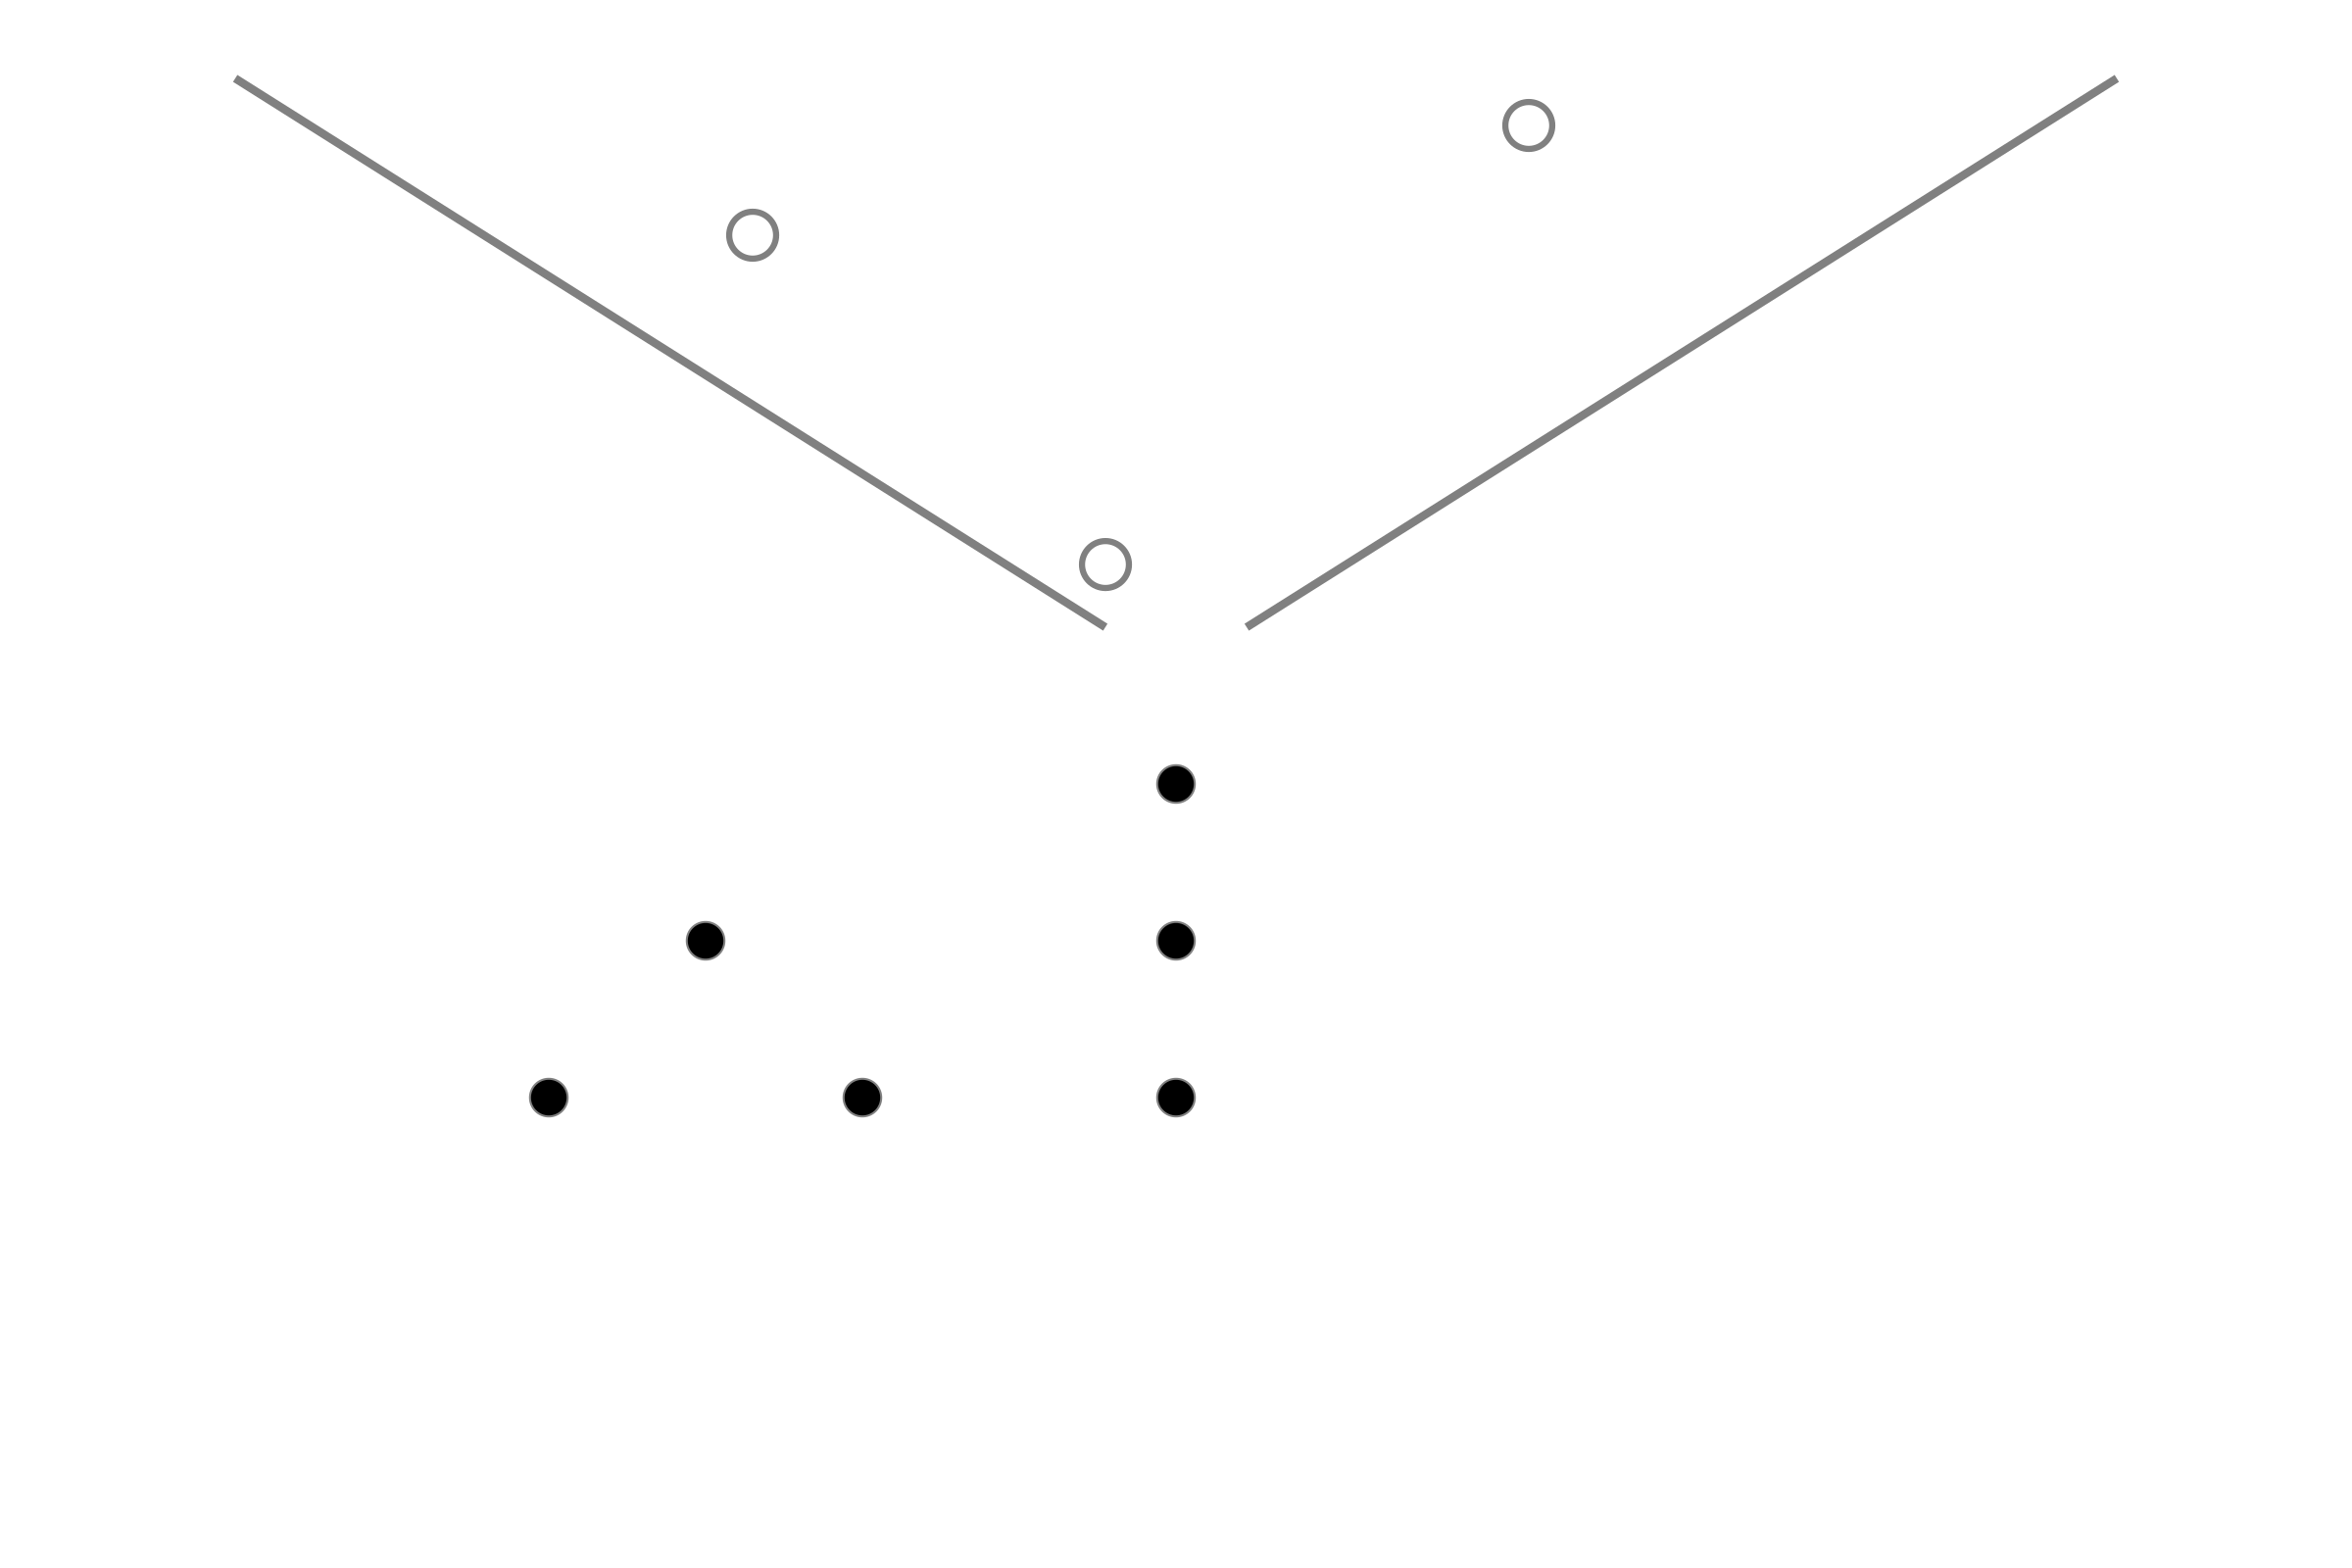
\includegraphics{_build/im/galton_box.png}
\caption{Schematic depiction of a Galton box; based on an image from
Wikimedia Commons.}\label{fig:galton_box}
}
\end{figure}

\hypertarget{sec:freq}{%
\section{Frequentist}\label{sec:freq}}

After introducing some common statistical notions in the previous
sections, we can now focus on linear models and their corresponding
statistical tests. From linear models, it is possible to formulate many
common tests, or very close approximations, including Pearson
correlations, t-tests and ANOVAs
(\protect\hyperlink{ref-lindelov2019common}{Lindeløv, 2019}). Note that
linear models are as valid in the Bayesian paradigm as in the
frequentist paradigm. However, here we focus on the combination with the
frequentists tests, which is why these models are listed under the
frequentist section.

In line with \protect\hyperlink{ref-bishop2006pattern}{Bishop}
(\protect\hyperlink{ref-bishop2006pattern}{2006}), generally, we can
write a linear model \(\text{lm}\) as

\[ \text{lm}(X_{v}, W_{m}) = w_0 + w_1 x_1 + ... + w_m x_v, \]

with input variables \(X_v\) and weights \(W_m\). Note that this means
that the data with \(n\) measurements can be stored in a \(n \times v\)
matrix. For the rest of this chapter, we assume that the errors are
Gaussian.

\hypertarget{one-sample}{%
\subsection{One sample}\label{one-sample}}

Say that you have a vector of sample values \passthrough{\lstinline!A!}
and want to test whether the mean of the population is \(x\). Lets
denote the mean of the population and sample respectively by \(\mu\) and
\(\mu_s\) and, for illustration purposes, lets generate some data:

\begin{lstlisting}
function one_sample_data()
    n = 12
    μ = 10
    σ = 3
    Random.seed!(1)
    A = rand(Normal(μ, σ), n)
    μ₀ = μ + 4
    (n, μ, σ, A, μ₀)
end
\end{lstlisting}

which is visualized in Figure~\ref{fig:plot_one_sample_data}.

\begin{figure}
\hypertarget{fig:plot_one_sample_data}{%
\centering
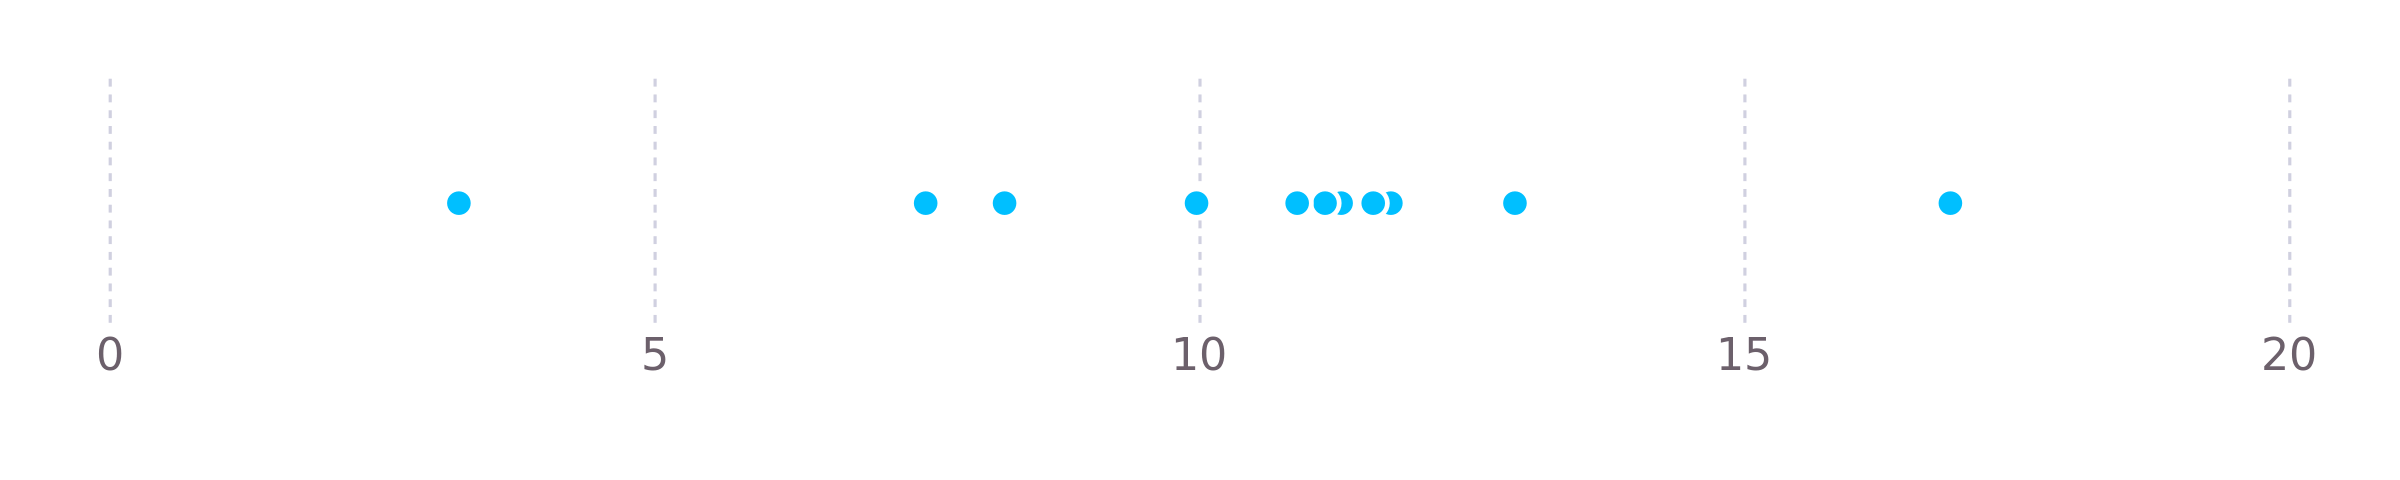
\includegraphics{_build/im/plot_one_sample_data.png}
\caption{12 points generated from a normal distribution with μ = 10 and
σ = 3.}\label{fig:plot_one_sample_data}
}
\end{figure}

Okay, so let's say that we want to know whether this data was generated
by a process having \(\mu_0\); this is our null hypothesis and we want
to check whether the data is significantly different, that is, we want
to test whether \(\mu \neq \mu_0\). A simple way to guess \(\mu\) is to
take the mean of the sample. However, these means on their own don't
provide much insight into \textbf{how} likely it is that
\(\mu = \mu_0\), see Figure~\ref{fig:plot_one_sample_data_mean}.

\begin{figure}
\hypertarget{fig:plot_one_sample_data_mean}{%
\centering
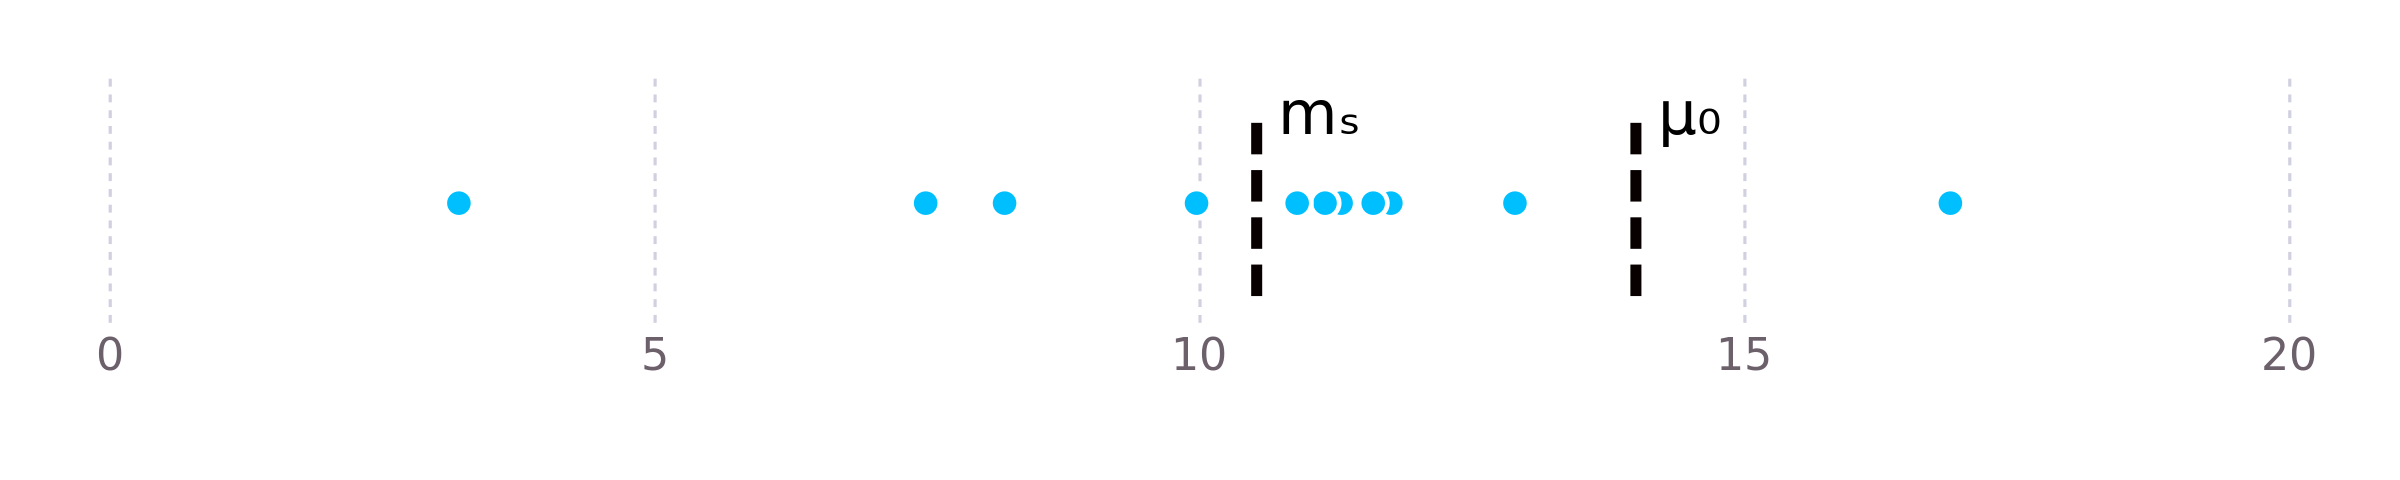
\includegraphics{_build/im/plot_one_sample_data_mean.png}
\caption{12 points generated from a normal distribution with μ = 10 and
σ = 3. Also, the sample mean mₛ and the null-hypothesis mean μ₀ are
shown.}\label{fig:plot_one_sample_data_mean}
}
\end{figure}

To estimate this, we can guess the distribution of the sample. As
already stated, we assume that data is generated from a normal
distribution and we can use the sample mean and standard deviation to
guess the distribution parameters. This distribution is depicted in
Figure~\ref{fig:plot_one_sample_data_distribution}.

\begin{figure}
\hypertarget{fig:plot_one_sample_data_distribution}{%
\centering
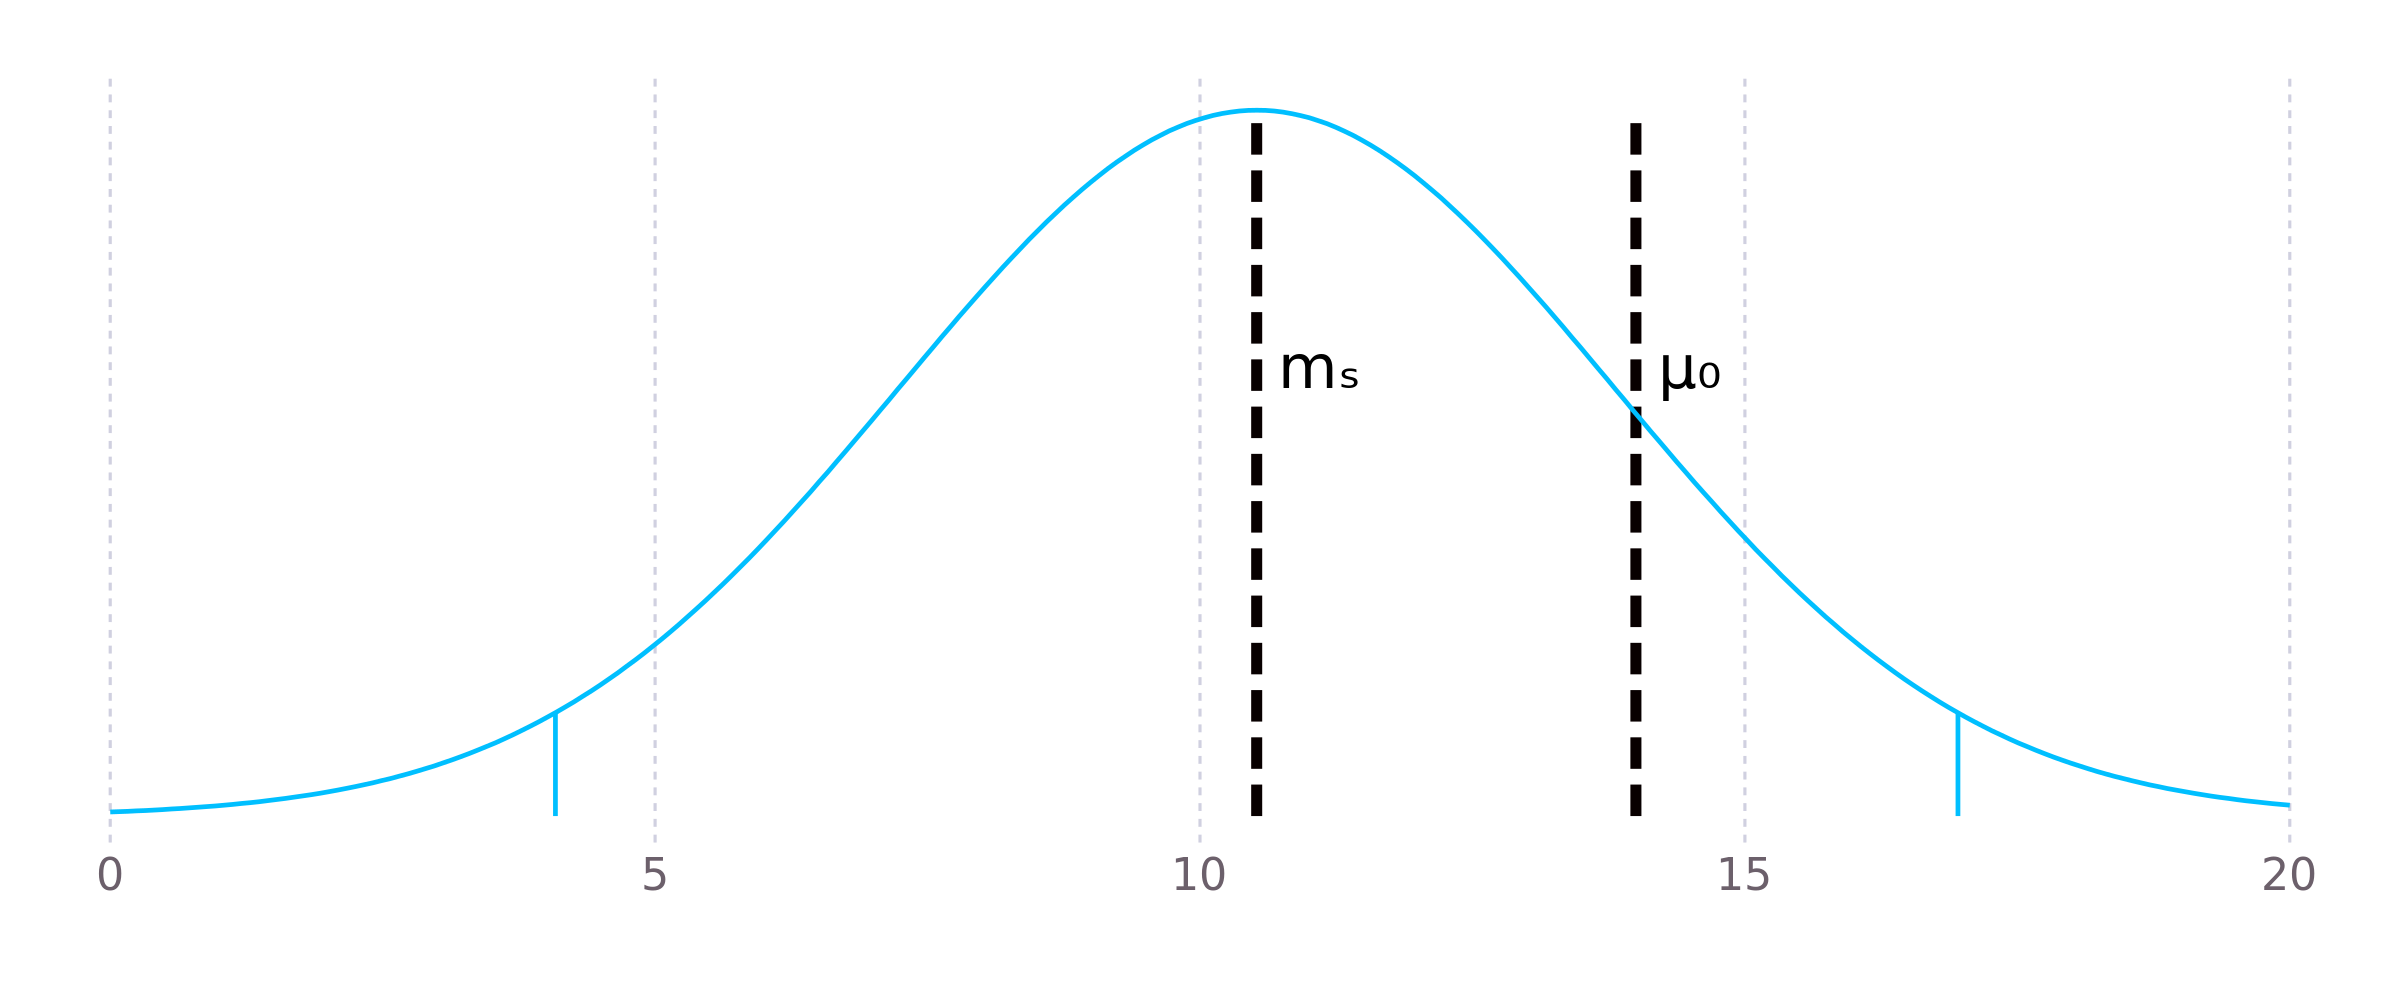
\includegraphics{_build/im/plot_one_sample_data_distribution.png}
\caption{Normal distribution for the sample mean and standard deviation.
The means for the sample mean mₛ and null-hypothesis μ₀ are indicated by
dashed black lines. The bounds for the 95\% confidence interval are
indicated by blue solid
lines.}\label{fig:plot_one_sample_data_distribution}
}
\end{figure}

Now that we have this distribution, we could come up with a formal
conclusion. For example, we can say that \(\mu = \mu_s\) if \(\mu_s\)
lies within the 95\% confidence interval of the estimated distribution.
Then, in this case, we would now conclude that the means do not
significantly differ.

Unfortunately, for small samples, the normal distribution isn't good
enough. This is due to the fact that \ldots{}

\[ \text{one\_sample}(X_v, W) = w_0 \]

\hypertarget{tbl:one_sample_tests}{}
\begin{longtable}[]{@{}rrrr@{}}
\caption{\label{tbl:one_sample_tests}Comparison of multiple models being
fitted on our sample data with alternative mean
\(\mu_0 = μ + 4 = 14\).}\tabularnewline
\toprule
model & p & lower & upper \\
\midrule
\endfirsthead
\toprule
model & p & lower & upper \\
\midrule
\endhead
t-test & 0.004 & 8.4 & 12.6 \\
\bottomrule
\end{longtable}

\hypertarget{sec:bayesian}{%
\section{Bayesian}\label{sec:bayesian}}

\hypertarget{sec:ci}{%
\chapter{Running computations automatically}\label{sec:ci}}

Continuous integrations (CI) and continous delivery (CD) allow software
developers to make fewer mistakes by validating code changes
automatically before applying them in the codebase. This is elaborated
on by
\href{https://about.gitlab.com/stages-devops-lifecycle/continuous-integration/}{GitLab}:
CI/CD is about ensuring ``the delivery of CI-validated code {[}\ldots{]}
via structured deployment pipelines.''

This sounds complex, but actually isn't. CI arose from the need to
validate code changes, in version control such as Git, automatically.
Upon each code change, a server takes the code and runs all the tests.
When the tests pass, you can be more sure that the changes are correct;
when the tests fail, you know that something is broken. This is
particulary helpful for code reviews when deciding whether the changes
should be merged in the codebase, see Figure~\ref{fig:green_ci}.

\begin{figure}
\hypertarget{fig:green_ci}{%
\centering
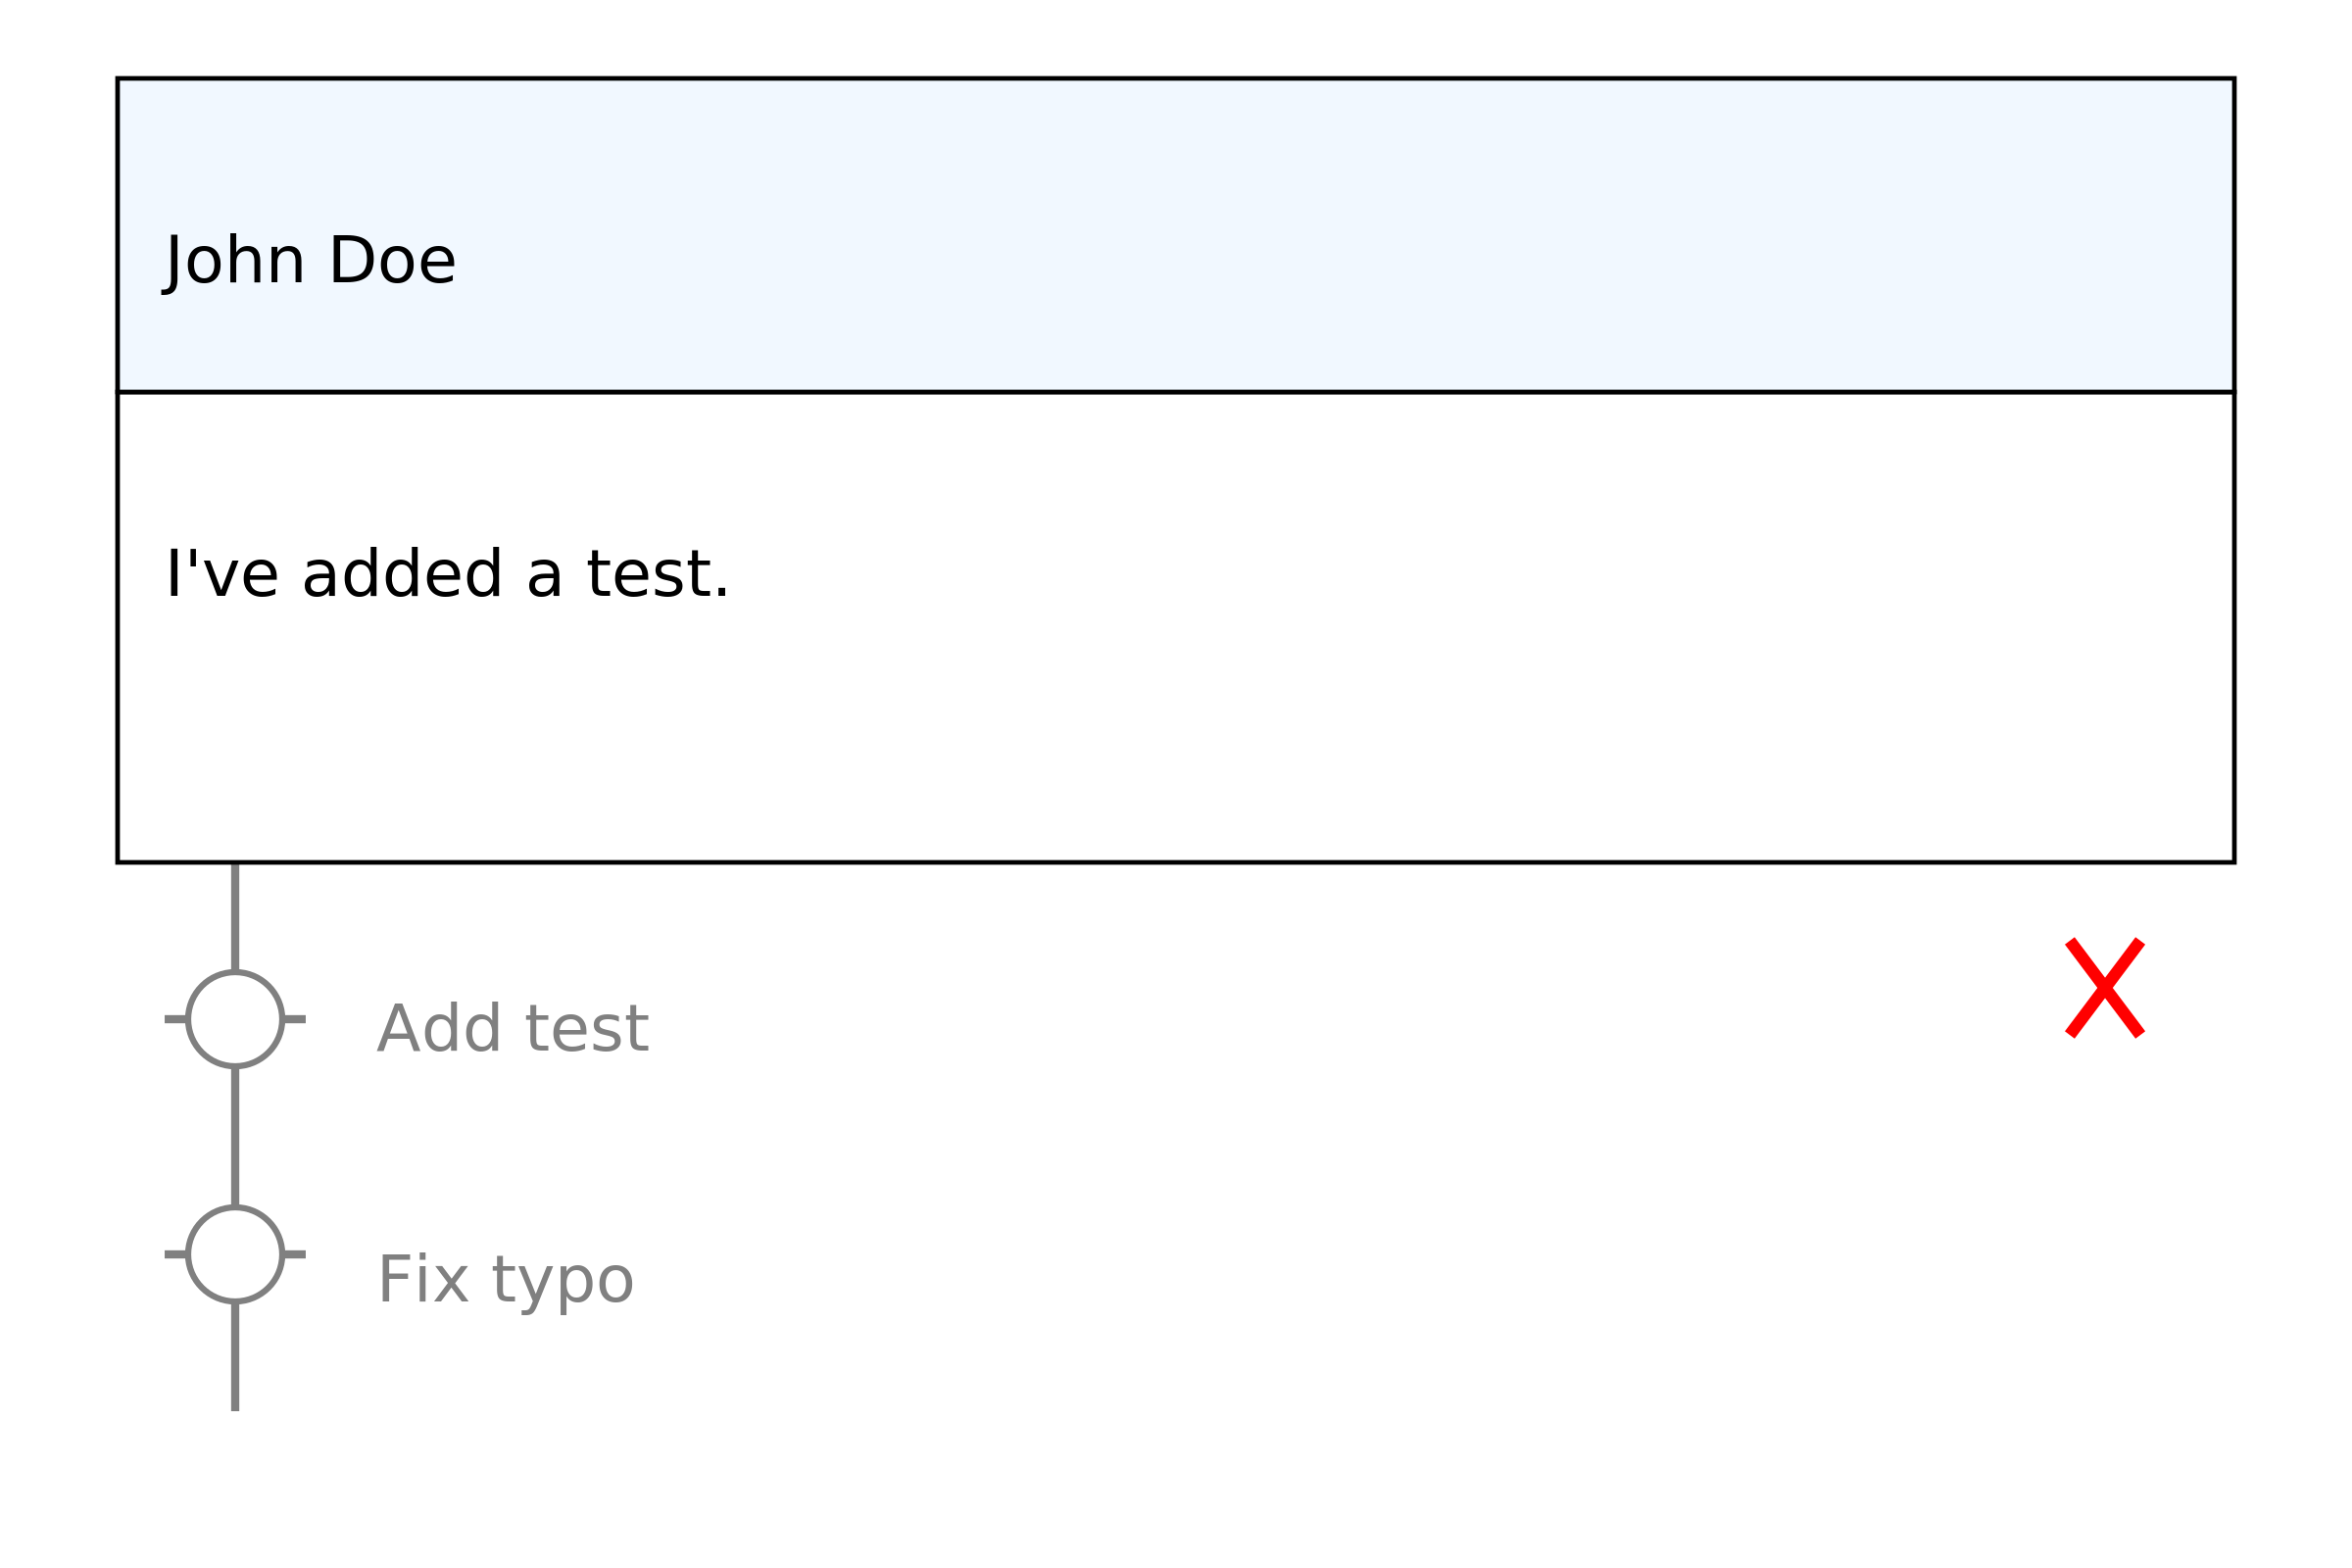
\includegraphics{_build/im/green_ci.png}
\caption{Simplified view of the GitHub interface for pull-requests. It
shows that John Doe did a failing commit and fixed it
afterwards.}\label{fig:green_ci}
}
\end{figure}

CD is also about running computations upon code changes. This time
however, the computations can do things like compiling the code into an
executable. The executable can then continuously be delivered to the
end-user, hence the name CD.

Interestingly enough, this idea is much more powerful than just CI/CD,
which is why GitHub calls it \href{https://github.com/home/}{GitHub
Actions} to ``automate anything.'' (You can read this as: \emph{automate
anything which can be controlled, directly or indirectly, from a
computer capable of running the GitHub runner}.) Like mentioned before,
upon each code change we can

\begin{itemize}
\tightlist
\item
  run tests, and/or
\item
  compile a program,
\end{itemize}

but we can also

\begin{itemize}
\tightlist
\item
  generate a website (like the one you're looking at right now),
\item
  generate a \href{https://github.com/hadley/r4ds}{book}, or
\item
  run a backup.
\end{itemize}

\textbf{TODO:} Add Compose.jl image here.

In essence, CI/CD and Workflows are about \textbf{linking computations
to text}.

(Actually, you can automate anything which can be managed by a GitHub
runner; this includes most, but not all, systems.)

\hypertarget{sec:appendix}{%
\chapter{Appendix}\label{sec:appendix}}

\hypertarget{versions}{%
\section{Versions}\label{versions}}

This website is built with Julia 1.6.0 and

\begin{lstlisting}
Books v0.4.2 `https://github.com/rikhuijzer/Books.jl#main#main`
Colors v0.12.7
Compose v0.9.2
DataFrames v1.0.1
Distributions v0.24.18
Gadfly v1.3.2
HypothesisTests v0.10.3
Pkg
Random
Statistics
\end{lstlisting}

Specifically, it is generated by
\url{https://github.com/rikhuijzer/tools} at commit
\passthrough{\lstinline!2fa8034758559bb93a19e4537501622d6455e05e!}.

\hypertarget{i3wm}{%
\section{i3wm}\label{i3wm}}

\hypertarget{references}{%
\chapter*{References}\label{references}}
\addcontentsline{toc}{chapter}{References}

\hypertarget{refs}{}
\begin{CSLReferences}{1}{0}
\leavevmode\hypertarget{ref-atkinson1991}{}%
Atkinson, R., \& John, E. (1991). \emph{{Interview with Elton John}}.
Laughing Stock Productions.

\leavevmode\hypertarget{ref-bishop2006pattern}{}%
Bishop, C. M. (2006). \emph{Pattern recognition and machine learning}.
springer.

\leavevmode\hypertarget{ref-deepmind2020alphago}{}%
DeepMind. (2020). \emph{AlphaGo}.
\url{https://deepmind.com/research/case-studies/alphago-the-story-so-far}

\leavevmode\hypertarget{ref-efron2016computer}{}%
Efron, B., \& Hastie, T. (2016). \emph{Computer age statistical
inference} (Vol. 5). Cambridge University Press.

\leavevmode\hypertarget{ref-greenberg2017hackers}{}%
Greenberg, A. (2017). Hackers say they've broken face ID a week after
IPhone x release. \emph{Wired, November}, \emph{12}.

\leavevmode\hypertarget{ref-harari2014sapiens}{}%
Harari, Y. N. (2014). \emph{Sapiens}. Bazarforlag AS.

\leavevmode\hypertarget{ref-harari2016homo}{}%
Harari, Y. N. (2016). \emph{Homo deus: A brief history of tomorrow}.
Random House.

\leavevmode\hypertarget{ref-hoare2014bet}{}%
Hoare, G. (2014). \emph{Always bet on text}.
\url{https://graydon2.dreamwidth.org/193447.html}

\leavevmode\hypertarget{ref-jordan2019artificial}{}%
Jordan, M. I. (2019). Artificial intelligence---the revolution hasn't
happened yet. \emph{Harvard Data Science Review}, \emph{1}(1).
\url{https://doi.org/10.1162/99608f92.f06c6e61}

\leavevmode\hypertarget{ref-lindelov2019common}{}%
Lindeløv, J. K. (2019). \emph{Common statistical tests are linear
models}. \url{https://lindeloev.github.io/tests-as-linear/}

\leavevmode\hypertarget{ref-loeliger2012version}{}%
Loeliger, J., \& McCullough, M. (2012). \emph{{Version Control with Git:
Powerful tools and techniques for collaborative software development}}.
O'Reilly Media, Inc.

\leavevmode\hypertarget{ref-pickett2018american}{}%
Pickett, J. P. (2018). \emph{The american heritage dictionary of the
english language}. Houghton Mifflin Harcourt.

\leavevmode\hypertarget{ref-smith2018mathematical}{}%
Smith, W. (2018). \emph{The mathematical symbols used in statistics}.
\url{https://ocw.smithw.org/csunstatreview/statisticalsymbols.pdf}

\leavevmode\hypertarget{ref-torvalds2005}{}%
Torvalds, L. (2005). \emph{{Kernel SCM saga..}}
\url{https://marc.info/?l=linux-kernel\&m=111288700902396}

\leavevmode\hypertarget{ref-wu2020towards}{}%
Wu, F., Lu, C., Zhu, M., Chen, H., Zhu, J., Yu, K., Li, L., Li, M.,
Chen, Q., Li, X., \& others. (2020). Towards a new generation of
artificial intelligence in china. \emph{Nature Machine Intelligence},
\emph{2}(6), 312--316. \url{https://doi.org/10.1038/s42256-020-0183-4}

\leavevmode\hypertarget{ref-yegge2012programmer}{}%
Yegge, S. (2012). \emph{{A Programmer's Rantings: On
Programming-Language Religions, Code Philosophies, Google Work Culture,
and Other Stuff}} (Note: also available at
https://sites.google.com/site/steveyegge2/tour-de-babel, Ed.). Hyperink
Inc.

\end{CSLReferences}

% \backmatter
\end{document}
